% %% file: template.tex = LaTeX template for article-like report 
%% init: sometime 1993
%% last: Feb  8 2015  Rob Rutten  Deil
%% site: http://www.staff.science.uu.nl/~rutte101/rrweb/rjr-edu/manuals/student-report/

%% First read ``latex-bibtex-simple-manual.txt'' at
%% http://www.staff.science.uu.nl/~rutte101/Report_recipe.html

%% Start your report production by copying this file into your XXXX.tex.
%% Small changes to the header part will make it an A&A or ApJ manuscript.

%%%%%%%%%%%%%%%%%%%%%%%%%%%%%%%%%%%%%%%%%%%%%%%%%%%%%%%%%%%%%%%%%%%%%%%%%%%%
%\documentclass{aa}   %% Astronomy & Astrophysics style class
\documentclass[a4paper]{report}
\usepackage[inner=2cm,outer=2cm]{geometry}
%\geometry{a4paper}
\usepackage{graphicx,url,twoopt}
\usepackage{subcaption}
\usepackage{enumitem}
\usepackage{amsmath}
\usepackage[varg]{txfonts}           %% A&A font choice
%\usepackage{hyperref}                %% for pdflatex
%%\usepackage[breaklinks]{hyperref}  %% for latex+dvips
%%\usepackage{breakurl}              %% for latex+dvips
%\usepackage{pdfcomment}              %% for popup acronym meanings
%\usepackage{acronym}                 %% for popup acronym meanings
\usepackage{calrsfs}
\DeclareMathAlphabet{\pazocal}{OMS}{zplm}{m}{n}

\usepackage{natbib}
% \hypersetup{
%   colorlinks=true,   %% links colored instead of frames
%   urlcolor=blue,     %% external hyperlinks
%   linkcolor=red,     %% internal latex links (eg Fig)
% }

 %\bibpunct{(}{)}{;}{a}{}{,}    %% natbib cite format used by A&A and ApJ
 
%\pagestyle{plain}   %% undo the fancy A&A pagestyle 


%%%%%%%%%%%%%%%%%%%%%%%%%%%%%%%%%%%%%%%%%%%%%%%%%%%%%%%%%%%%%%%%%%%%%%%%%%%%
\begin{document}  

%\twocolumn[]
%\onecolumn
%%%%%%%%%%%%%%%%%%%%%%%%%%%%%%%%%%%%%%%%%%%%%%%%%%%%%%%%%%%%%%%%%%%%%%%%%%%%
\section{Introduction}\label{sec:introduction}
%%%%%%%%%%%%%%%%%%%%%%%%%%%%%%%%%%%%%%%%%%%%%%%%%%%%%%%%%%%%%%%%%%%%%%%%%%%%
In this project I am following the algorithm presented in Callin (2005)[1] for simulating the cosmic microwave background.  
This is the final part of the project.

In the first part I set up the background cosmology of the universe, and made a function that could find the conformal time as a function of $x$. In the second part I computed the electron fraction, electron density, optical depth and visibility function for times around and during recombination. The third part use the two previous to compute the density perturbations, and velocities of dark matter and baryons. This also included the temperature multipoles $\Theta_l$.

This final part combines all of these quantities to compute the final CMB power spectrum.

As previously done I will continue building on the skeleton code provided.

%%%%%%%%%%%%%%%%%%%%%%%%%%%%%%%%%%%%%%%%%%%%%%%%%%%%%%%%%%%%%%%%%%%%%%%%%%%%
\section{Equations}\label{sec:Equations}
%%%%%%%%%%%%%%%%%%%%%%%%%%%%%%%%%%%%%%%%%%%%%%%%%%%%%%%%%%%%%%%%%%%%%%%%%%%%
In this final part of the project we finally combine everything from the previous projects into the final CMB power spectrum. This is done by a few equations, the first of which is the Transfer function defined
\begin{equation}
 \Theta_l(k,x=0)=\int^0_{-\infty} \tilde{S}(k,x)j_l[k(\eta_0-\eta)]dx,
\end{equation}
where $j_l$ is the spherical Bessel functions, and S is the source function defined
\begin{equation}
 \tilde{S}(k,x) = \tilde{g}\bigg[\Theta_0+\Psi+\frac{1}{4}\Pi\bigg]+e^{-\tau}[\Psi^\prime-\Phi^\prime]-\frac{1}{ck}\frac{d}{dx}(\pazocal{H}\tilde{g}v_b) +\frac{3}{4c^2k^2}\frac{d}{dx}\bigg[\pazocal{H}\frac{d}{dx}(\pazocal
{H}\tilde{g}\Pi) \bigg].
\end{equation}
The only variable not explained earlier in this equation is $\Pi = \Theta_2 +\Theta_0^P+\Theta_2^P$, which contain two not previously used variables $\Theta_0^P$, and $\Theta_2^P$. These two are related to the polarization of the temperature multi poles. Since we chose to not include polarization and neutrinos in the last part of the project, these two can be set to zero, which means that for our case $\Pi = \Theta_2$.

The Source function deserves a bit of explaining. Its job is, as expected from its name, to source the spectrum for all $k$ modes at all $x$ values. It consist of four distinct terms each describing different effects. 

The first is the local monopole weighted by the visibility function $\tilde{g}$, this term also includes the fact that the photons climb out of a gravitational potential $\Psi$ and a small correction term $\Pi$. This redshifting of the photons is known as the Sachs-Wolfe effect. 

The second term is the integrated Sachs-Wolfe effect. This term takes care of the change due to changing gravitational fields the photons encounter on their way from the last scattering surface to us today.

The third term corrects for the doppler effect, and the fourth term FIGURE OUT WHAT THIS IS FIGURE OUT WHAT THIS IS FIGURE OUT WHAT THIS IS FIGURE OUT WHAT THIS IS FIGURE OUT WHAT THIS IS FIGURE OUT WHAT THIS IS FIGURE OUT WHAT THIS IS FIGURE OUT WHAT THIS IS FIGURE OUT WHAT THIS IS 


This is then multiplied by the spherical bessel functions which projects this three dimensional field onto the surface of a sphere. This gives us the so-called Transfer function. Note however that this only takes care of the $x$ values. We still need to account for all $k$ modes, and all directions. And furthermore we have not yet included the spectrum left over by inflation which is what we started out with. (This is fine as was discused previously since we use linearized equations.)

The full CMB power spectrum then reads 
\begin{equation}
 C_l = \int\frac{d^3k}{(2\pi)^3}P(k)\Theta_l^2(k)
\end{equation}
Here we finally scale by $P(k)$. Recall that we set $\Phi = 1$ as the initial condition, instead of $\Phi = P(k)$. This is fine since we are working with linearized equations. If the reader wants to use higher order equations this needs to be taken into account from the beginning.

Furthermore, if we consider that most inflationary models predict a Harrrison-Zel'dovich spectrum where 
\begin{equation}
 \frac{k^3}{2\pi^2}P(k) = \bigg(\frac{ck}{H_0}\bigg)^{n-1}
\end{equation}
holds, we can write the CMB power spectrum as
\begin{equation}
  C_l = \int_0^\infty\bigg(\frac{ck}{H_0}\bigg)^{n_s-1}\Theta_l^2(k)\frac{dk}{k}.
\end{equation}
Here $n_s$ is the spectral index, which according to the latest data from Planck[2] is $n_s = 0.968\pm0.006$.
Since the overall trend of the power spectrum is to drop as $l^{-2}$, it is a good idea to plot the spectrum in units of $l(l+1)/2\pi$ in $\mu K^2$. This makes it easier to see features in it. So far we have not normalized the spectrum in any way. Since we want to compare it to the observed spectrum, we simply say that the maximum is $5775\mu K^2$, when measured in the above units.

With this we should now get a power specturm that can be fitted to the data, making it possible to estimate the density components of the universe.

%%%%%%%%%%%%%%%%%%%%%%%%%%%%%%%%%%%%%%%%%%%%%%%%%%%%%%%%%%%%%%%%%%%%%%%%%%%%
\section{Implementation}\label{sec:Imp}
%%%%%%%%%%%%%%%%%%%%%%%%%%%%%%%%%%%%%%%%%%%%%%%%%%%%%%%%%%%%%%%%%%%%%%%%%%%%
From the earlier projects we have arrays with $x$, and $k$ values. We use these to calculate the source function. The result is then splined onto a high resolution grid in $x$ and $k$. We also see in the Transfer function that we want values for $j_l$ for a combination of $k$ and $\eta(x)$ values. It turns out that these numbers are in the range $[0,3400]$. Thus we sample $5400$ values linearly in this range, and then spline that so we can find arbitrary values in between them. 

We now have the spherical bessel functions and Source functions for all values in our high resolution $k$ and $x$ grid making it possible to calculate the Transfer function. The $x$ and $k$ grids have $5000$ values in the same range as earlier, only this time the steps are linear through $x$, while $k$ is quadratic like before.

To find the Transfer function we need a numerical integration method. I have chosen to use the trapezoidal method. The integration limits go from $-\infty$ to $0$. Luckily for us the Source function is zero for almost all times except around the last scattering surface. Because of this we simply set the lower integration limit to a very low $x$ value still inside our grid.

The next step is to calculate $C_l$. This is done in precisely the same fashion. The only difference is the integration limits. We integrate over the $5000$ $k$ values in our grid. For information on why we only need this many k values for the integration see Callin(2005)[1]. In short it has to do with getting a good amount of values between each oscillation of the  Bessel function. 



%%%%%%%%%%%%%%%%%%%%%%%%%%%%%%%%%%%%%%%%%%%%%%%%%%%%%%%%%%%%%%%%%%%%%%%%%%%%
\section{Results}\label{sec:results}
%%%%%%%%%%%%%%%%%%%%%%%%%%%%%%%%%%%%%%%%%%%%%%%%%%%%%%%%%%%%%%%%%%%%%%%%%%%%
Underway through the workings of the program I have plotted various quantities to make sure that they return sensible results. An example is the integrand in the Transfer function (figure \ref{fig:integrand}).

\begin{figure}[ht]
 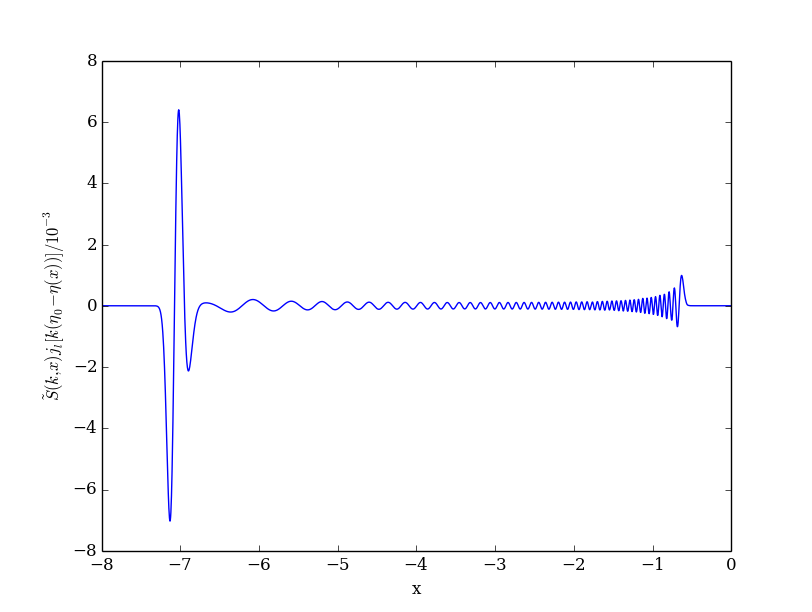
\includegraphics[width=\textwidth]{integrand.png}
 \caption{The integrand in the Transfer function integral for $l= 100$, and $k \approx160H_0/c$. The source function gives a spike around recombiniation, while the Bessel function makes it oscillate at late times. This is sensible.}
 \label{fig:integrand}
\end{figure}

Another useful quantity is the Transfer function. This has been plotted for six different k values in figure \ref{fig:transfer}.
\begin{figure}[ht]
 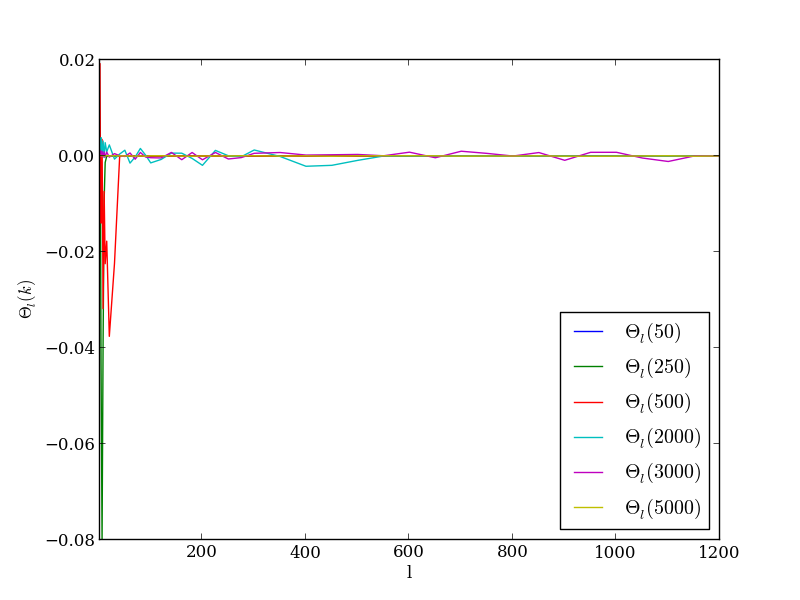
\includegraphics[width=\textwidth]{transfer.png}
 \caption{The Transfer function for k number 50,250,500,2000,3000, and 5000. Note that this does not correspond to the actual value of k. If the reader is interested in the actual k value he/she will have to use equation 14 presented in part 3 of the project for each of the k values. }
 \label{fig:transfer}
\end{figure}

We should also make sure that the integrand in the power spectrum integral behaves appropriately. This can be seen in figure \ref{fig:integ}
\begin{figure}[ht]
 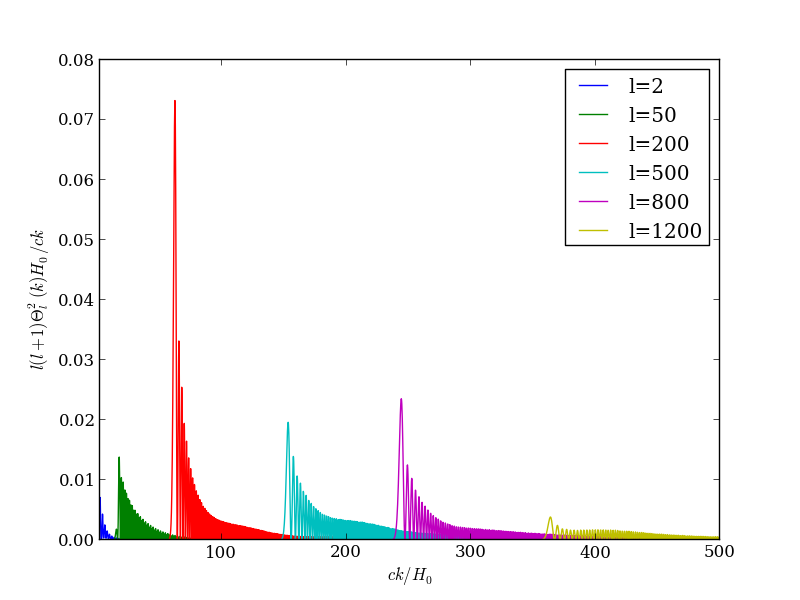
\includegraphics[width=\textwidth]{integ.png}
 \caption{}
 \label{fig:integ}
\end{figure}

Finally, the CMB power spectrum can be seen in figure \ref{fig:Cl}.
\begin{figure}[ht]
 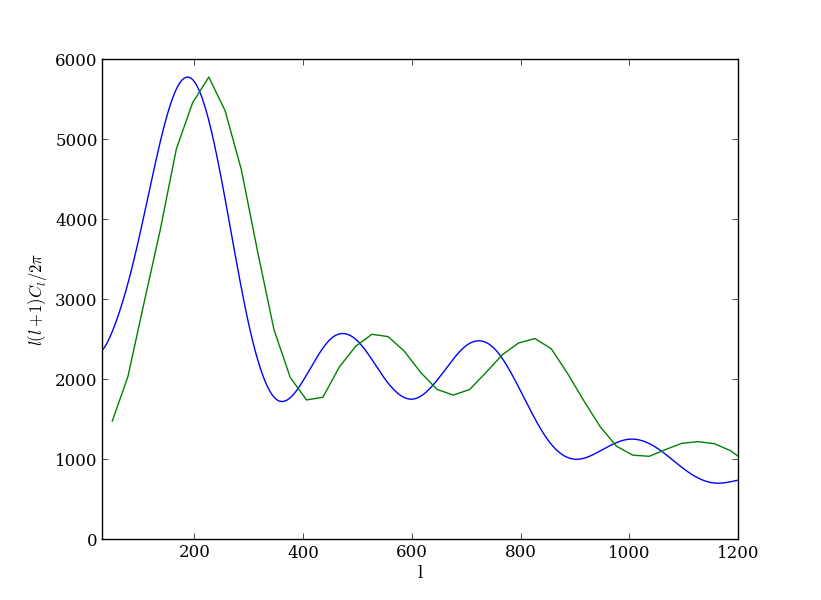
\includegraphics[width=\textwidth]{Cl.png}
 \caption{The CMB power spectrum. Computed in blue, and observed data in green.}
 \label{fig:Cl}
\end{figure}


%%%%%%%%%%%%%%%%%%%%%%%%%%%%%%%%%%%%%%%%%%%%%%%%%%%%%%%%%%%%%%%%%%%%%%%%%%%%
\section{Conclusions}\label{sec:Conc}
%%%%%%%%%%%%%%%%%%%%%%%%%%%%%%%%%%%%%%%%%%%%%%%%%%%%%%%%%%%%%%%%%%%%%%%%%%%%
We have seen that we can get fairly close to the observed power spectrum even though we did not include neutrinos or polarization. 


Unfortunately time did not allow me to use a Metropolis algorithm to estimate the values of the various cosmological parameters. This is something I will have to do on my own time afterwards. This is unfortunate as this would have been the icing on the cake.


%%%%%%%%%%%%%%%%%%%%%%%%%%%%%%%%%%%%%%%%%%%%%%%%%%%%%%%%%%%%%%%%%%%%%%%%%%%%
\section{References}
%%%%%%%%%%%%%%%%%%%%%%%%%%%%%%%%%%%%%%%%%%%%%%%%%%%%%%%%%%%%%%%%%%%%%%%%%%%%
\begin{enumerate}[label= {[}\arabic*{]} ]
 \item P. Callin, astro-ph/0606683
 \item P. A. R. Ade et al. [Planck Collaboration], arXiv:1502.02114 [astro-ph.CO].
 
\end{enumerate}

\onecolumn 
%%%%%%%%%%%%%%%%%%%%%%%%%%%%%%%%%%%%%%%%%%%%%%%%%%%%%%%%%%%%%%%%%%%%%%%%%%%%
\section{Source code}\label{sec:files}
%%%%%%%%%%%%%%%%%%%%%%%%%%%%%%%%%%%%%%%%%%%%%%%%%%%%%%%%%%%%%%%%%%%%%%%%%%%%
The source code for the function made for computing the high resolution source function in evolution\_mod.f90 is included as well as the file cl\_mod.f90 file used for computing the final power spectrum is included for inspection. This file depends on all files previously used in the three earlier parts of the project.



%%%%%%%%%%%%%%%%%%%%%%%%%%%%%%%%%%%%%%%%%%%%%%%%%%%%%%%%%%%%%%%%%%%%%%%%%%%%
%\begin{acknowledgements}
%\end{acknowledgements}

\end{document}